\documentclass[11pt,a4paper]{article}
\usepackage{ls}
\usepackage[russian,german]{babel}

\title{Handreichung zum Einsatz des TRIZ-Trainers}

\author{Hans-Gert Gr\"abe}

\newcommand{\normbox}[1]{{\fboxsep2mm\fbox{\rule[-4pt]{0pt}{12pt}#1}}}

\date{10. April 2021}

\begin{document}
\maketitle
\tableofcontents
\newpage

\section{Allgemeines}

Im Rahmen einer internationalen Kooperation nutzen wir im
TRIZ-Online-Praktikum den von \emph{Target Invention} in Minsk (Belarus)
entwickelten TRIZ-Trainer \url{https://triz-trainer.com} als Lernmittel.  Der
TRIZ-Trainer ist eine leichtgewichtige Version zur Unterstützung von Blended
Learning\footnote{\url{https://de.wikipedia.org/wiki/Integriertes_Lernen}} als
methodischem Praktikumskonzept im Sinne eines angeleiteten Selbststudiums.

Der TRIZ-Trainer konzentriert sich auf die Basiskonzepte des Einsatzes von
TRIZ an ausgewählten praktischen Beispielen -- die Analyse und Modellierung
der jeweiligen Problemsituation, die Identifizierung und Lokalisierung
entsprechender Wirkfaktoren und Widersprüche sowie die strukturierte
Verwendung entsprechender Lösungsschemata.  Zur Einarbeitung und zum besseren
Verständnis der Thematik wird neben dem ausführlichen Hilfesystem des
TRIZ-Trainers das Lehrbuch \cite{KS2017} empfohlen.

Der TRIZ-Trainer ist selbst noch in Entwicklung.  Im Rahmen unserer
Kooperation unterstützen wir die Minsker Kollegen bei der Aktualisierung der
deutschsprachigen Version.  Neue oder noch nicht übersetzte Teile werden zügig
über das redaktionelle System der Anwendung konsolidiert.  Bitte informieren
Sie uns zeitnah über entsprechende Probleme.

\section{TRIZ als Problemlösemethodik}

Die TRIZ-Methodik kommt als Problemlösemethodik vor allem dort zum Einsatz, wo
Standardlösungen oder durch einfache Ingenieurskunst zu findende
Lösungsansätze nicht greifen.  Grund des Versagens ist meist ein
\emph{Hindernis}, das einer „einfachen“ Lösung im Weg steht und sich als
\emph{Widerspruch} manifestiert (Bild 1). 

\begin{figure}[ht]\centering
    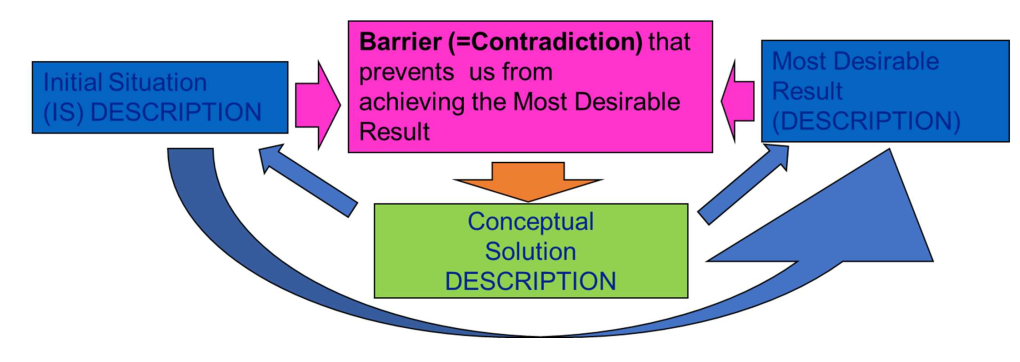
\includegraphics[width=.8\textwidth]{Basics.png}\\
    \textbf{Bild 1:} Das TRIZ Vorgehensmodell
\end{figure}

Im Zuge der Modellierung wird dieser Widerspruch oft als \emph{Konflikt}
identifiziert, wo ein (aus Sicht des Systemzwecks) nützlicher Effekt nicht
ohne einen schädlichen weiteren Effekt zu haben ist, sowie die \emph{operative
  Zone} (in Raum und Zeit) genauer bestimmt, in welcher der Konflikt auftritt.
Im TRIZ-Ansatz wird versucht, derartige Konflikte nicht durch Kompromisse zu
lösen, sondern zu prinzipiellen innovativen Ansätzen zu kommen.

\emph{Beispiel:} Ein Teeglas wird mit heißem Tee gefüllt (nützlicher Effekt
„heißer Tee schmeckt“, schädlicher Effekt „beim Anfassen verbrenne ich mir die
Finger“).  Die Kompromisslösung „lauwarmer Tee“ stellt niemanden zufrieden.
Mit TRIZ analysieren wir, wo der Konflikt auftritt (an der Glaswand beim
Anheben des Glases zum Trinken). Typischer Lösungsansatz ist hier das
Separationsprinzip -- kann man das Ganze räumlich oder zeitlich trennen?
Funktion des Glases: Behälter für den Tee, also kann nur was mit der Hand
geändert werden. Fasse das Glas mit einem Handschuh an (der wirkt
wärmedämmend), oder mit einer Grillzange (Abstand). Oder verwende einen
Teeglashalter (perfektioniert die Idee mit der Grillzange).  Oder pappe den
Henkel des Teeglashalters gleich an das Teeglas (schon perfektere räumliche
Separation am Teeglas selbst; „Trimmen“ des Teeglashalters).  Oder analysiere
genauer: Glaswand muss \emph{innen} heiß und \emph{außen} kalt sein.  Stelle
also das Behältnis aus wäredämmendem Material her -- der Coffee-To-Go-Becher
ist erfunden.

\begin{figure}[ht]\centering
    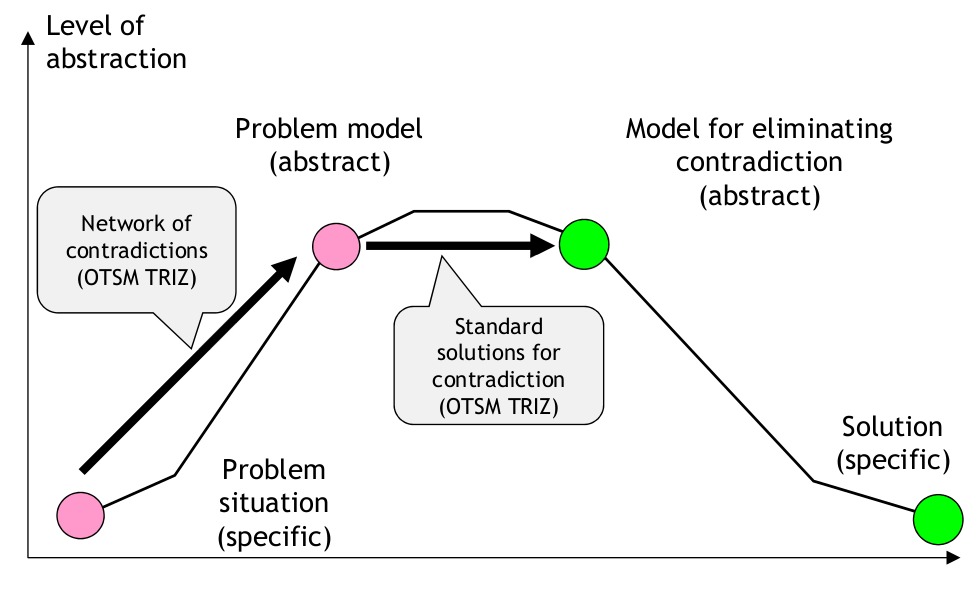
\includegraphics[width=.8\textwidth]{HillModel.png}\\
    \textbf{Bild 2:} Das TRIZ Hügelmodell
\end{figure}
Die TRIZ-Methodik orientiert sich dabei am Hügelschema (Bild 2)
\begin{itemize}
\item [1)] Modellierung des gegebenen Problems (Aufbau und Ablaufstruktur des
  Systems, raum-zeitliche Eingrenzung der Problemregion im Modell als
  \emph{operative Zone}, Identifizierung der Widerspruchsstruktur des
  Problems), 
\item [2a)] Identifizierung der abstrakten Problemstruktur, der verfügbaren
  Ressourcen und Auswahl der für eine Lösung geeigneten TRIZ-Werkzeuge
  (\emph{Aufgabenmodell}),
\item [2b)] Anwendung der Werkzeuge, um eine abstrakte Lösung zu entwickeln
  (\emph{Lösungsmodell}),
\item [3)] Instrumentierung der Lösung mit geeigneten Ressourcen und Ableitung
  eines oder mehrerer konkreter Lösungsvorschläge.
\end{itemize}

\section{Der Workflow im TRIZ-Trainer}

\subsection{Registrierung und Aktivierung des Accounts}

Das Anlegen und Aktivieren der Accounts und die Zuweisung der Rolle
\emph{Student} erfolgt zentral durch die Praktikumsleitung, wenn die
Accountgebühr eingezahlt wurde.  Der Account ist zeitlich befristet.

Die weiteren Ausführungen gehen davon aus, dass Sie sich am System
authentifiziert haben (Menü ganz rechts) und in der Rolle \emph{Student}
agieren.  Die beiden Felder daneben (mit den Tooltips \emph{Notifications} und
\emph{Settings}) dienen der Steuerung Ihrer Aktivitäten. Über das Feld
\emph{Notifications} haben Sie Zugriff auf Ihre bisherigen Lösungsversuche.

Die deutsche Version aktiviert sich automatisch an Hand der Spracheinstellung
Ihres Browsers, gegebenenfalls kann dies auch im Auswahlfeld im Seitenfuß
umgeschaltet werden.

Ich bin Ihnen als Trainer zugewiesen und kann somit Ihre Aktivitäten
verfolgen, kommentieren und bewerten.

\subsection{Den Bearbeitungsprozess starten}

Nach dem Einloggen gehen Sie auf die Seite \emph{Aufgaben} und beginnen, die
Aufgaben zu lösen, die Sie mögen.  Es empfiehlt sich natürlich, vorher die
Hinweise unter \emph{Lösungsprozess} und diese Handreichung genauer zu
studieren.  Im Hilfesystem des TRIZ-Trainers werden zu jedem Schritt im
Lösungsprozess ausführliche Hinweise gegeben, was im jeweiligen Schritt zu tun
ist und wie an die Teilaufgabe herangegangen werden sollte.

Es werden Ihnen mehrere Aufgabenserien angeboten, was aber eine eher
technische Einteilung ist.  Das Lösen der Aufgaben setzt eine gewisse
Vertrautheit mit der TRIZ-Methodik voraus, die \textbf{im Zuge eines
  Selbststudiums} vorab zu erwerben ist und im Laufe des Praktikums vertieft
werden soll.  Es geht also nicht darum, \emph{die Aufgaben irgendwie zu
  lösen}, sondern an diesen Beispielen \textbf{die Anwendung der TRIZ-Methodik
  und den Einsatz angemessener TRIZ-Werkzeuge} zu üben und zu perfektionieren.
Hinweise dazu finden Sie über die Links ins Hilfesystem oder -- in kurzer Form
-- in den Tooltipps zu jedem einzelnen Schritt. Schauen Sie sich auch die
\emph{Beispielaufgaben} an.

\subsection{Bearbeiten, Einreichen, Bewerten} 

Alles beginnt damit, dass Sie mindestens ein Zeichen in die Vorlage einer
Aufgabe einfügen, um das Problem zu lösen. Beim automatischen Speichern
wechselt die Aufgabe in den Status \emph{wird gelöst} und wird auf der Seite
\emph{Ergebnisse} dem zugeordneten Trainer angezeigt. Der Trainer kann so
bereits sehen, welche Aufgaben Sie zu lösen begonnen (aber noch nicht beendet)
haben und kann den Fortschritt Ihrer Arbeit verfolgen. Der Trainer kann in
diesem Stadium bereits Kommentare zu den einzelnen Schritten geben.

Ist Ihre Lösung komplett, klicken Sie auf die Schaltfläche \emph{Zur
  Überprüfung einreichen} und reichen damit die Aufgabe zur Bewertung ein.
Der Trainer analysiert Ihre Lösung, kommentiert einzelne Schritte und trifft
die Entscheidung, die Lösung anzuerkennen (Status \emph{angerechnet}) oder zur
Überarbeitung zurückzugeben (Status \emph{zu überarbeiten}).  Kommentare trage
ich grundsätzlich in die offen sichtbaren Felder „Kommentare des Trainers“
ein.

Ihnen werden der Status der Lösung und die Kommentare des Trainers sowohl über
die internen \emph{Notifications} als auch per E-Mail mitgeteilt.  Wenn die
Aufgabe zur Überarbeitung zurückverwiesen wird, ist sie von Ihnen erneut zu
bearbeiten.  Wenn die Lösung akzeptiert wurde, ist die Bearbeitung der Aufgabe
beendet.

Es gibt kein „richtig“ oder „falsch“, sondern die Qualität der Lösung
entsprechend der Methodik wird begutachtet.

\section{Zur Methodik}

Primäres Ziel des Einsatzes des TRIZ-Trainers ist dessen Einbettung in den
Kontext eines Flipped-Classroom-Konzepts, in dem -- einem Spiralmodell des
Kompetenzzuwachses folgend -- praktische Problemstellungen zur Beschäftigung
mit Theorie anregen und umgekehrt die studierte Theorie Ihre Fertigkeiten zum
Lösen praktischer Problemstellungen verbessert. Dazu wird mit
AIPS-2015\footnote{Die Abkürzung steht für \foreignlanguage{russian}{Алгоритм
    Исправления Проблемных Ситуаций} (Algorithmus zur Verbesserung
  problematischer Situationen).}  eine spezielle in Minsk entwickelte
algorithmische Version der TRIZ-Methodik eingesetzt, die den Lösungsprozess
entsprechend dem Hügelschema in drei Phasen unterteilt.

Die Aufgaben sind so weit heruntergebrochen, dass sie (meist) nur \emph{eine}
widersprüchliche Grundsituation enthalten bzw. nur auf \emph{eine} solche
fokussiert wird.  Der gelegentlich vorhandene Interpretationsspielraum ist
stets so zu verstehen ist, dass
\begin{itemize}[noitemsep]
\item in der \emph{konkret betrachteten} Situation
\item eine der Situation angemessene \emph{konstruktive ingenieur-technische
  Lösung}
\item mit möglichst wenig zusätzlichen Hilfsmitteln und 
\item möglichst geringer Modifikation des vorhandenen Systems
\end{itemize}
zu finden ist.

Die meisten Aufgaben beziehen sich auf ein \emph{abgegrenztes technisches
  System} mit einer \emph{problematischen Komponente} (Boot mit Mast, Kipper
mit Auspuffanlage, Motorradfahrer mit Schutzbrille, Auto mit zugefrorener
Scheibenwaschanlage usw.). Das technische System erfüllt einen gewissen Zweck,
die problematische Komponente hindert es daran, diesen Zweck unter gewissen
Einsatzbedingungen gut oder überhaupt zu erfüllen.

In der \textbf{ersten Phase}, der \emph{Analyse der Problemsituation}, ist
eine genaue Modellierung der gegebenen Situation auszuführen. Dabei ist sowohl
das System als auch die problematische Komponente genauer zu modellieren.  Das
Modell des Systems dient dazu, die verfügbaren Ressourcen zu bestimmen, das
Modell der problematischen Komponente bringt die genaueren
Problemzusammenhänge ans Licht.  Dieser Teil endet mit der Formulierung
verschiedener Hypothesen, wie die analysierte widersprüchliche Situation
aufgelöst werden kann, aus denen eine für die zweite Phase als \emph{Aufgabe}
formuliert und genauer analysiert wird.  Bitte beachten Sie die präzisierenden
Ausführungen zu dieser Phase im Abschnitt 4 dieser Handreichung.

Am \textbf{Ende der ersten Phase} sind aus den Modellierungen des Systems
sowie der problematischen Komponente eine oder mehrere abstrakte
Konfliktlösungshypothesen\footnote{\textbf{Vermeiden Sie möglichst folgenden
    Anfängerfehler:} Die Hypothesen sind zu konkret und stark mit
  Brainstorming durchsetzt, fokussieren auf scheinbar „offensichtliche“
  Lösungen. Dieses Phänomen hat in der TRIZ einen eigenen Namen:
  „psychologische Trägheit“.} entwickelt und eine davon für die weitere
Bearbeitung als \emph{Bedingungen der Aufgabe} ausgewählt. Zugleich wird durch
die Modellierung implizit der \emph{Kontext} bestimmt, in dem sich die weitere
Lösungssuche abspielt.

In der \textbf{zweiten Phase}, der \emph{Formulierung und Lösung der
  abstrakten Aufgabe}, ist diese präzisierte Aufgabe nach einem (oder
mehreren) von vier \emph{Aufgabenmodellen} entsprechend der für das jeweilige
Aufgabenmodell vorgesehenen Methodik genauer zu analysieren:
\begin{itemize}[noitemsep]
\item Bedingungen in der operativen Zone (wenn eine Systemkomponente im
  Problembereich ergänzt oder modifiziert werden soll; typische
  TRIZ-Werkzeuge: \emph{X-Komponente} und \emph{funktionale Modellierung}),
\item Wirkungen in der operativen Zone (wenn Wirkungen im Problembereich
  modifiziert werden sollen; typische TRIZ-Werkzeuge: \emph{SF-Modelle} und
  \emph{Inventive Standards}), 
\item Technischer Widerspruch (wenn widersprüchliche technische Anforderungen
  aufzulösen sind; typische TRIZ-Werkzeuge: \emph{Wirkungspaar} und ein
  geeignetes \emph{TRIZ-Prinzip}),
\item Physikalischer Widerspruch (das technische Widerspruchspaar lässt sich
  auf widersprüchliche Anforderungen an \emph{einen} physikalischen Parameter
  reduzieren; dafür typische TRIZ-Werkzeuge: \emph{Separationsprinzipien},
  \emph{TRIZ-Prinzipien}).
\end{itemize}
Die Anwendungsgebiete der vier Aufgabenmodelle sind im Abschnitt „Lösen der
herausgearbeiteten Aufgabe“ des Hilfesystems hinreichend detailliert
erläutert.

Weiter werden die Ressourcen identifiziert, die für eine Lösung der Aufgaben
prinzipiell zur Verfügung stehen.


Das (abstrakte) Aufgabenmodell und die dazu auszuwählenden TRIZ-Werkzeuge
werden im Zuge der Anwendung einer geeigneten \emph{Umwandlungsmethode} in ein
(abstraktes) \emph{Lösungs\-modell} transformiert, das -- mit geeigneten
Ressourcen instrumentiert -- zu einer Lösungsidee weiter ausgebaut werden
kann.  Dieser Teil ist im Hilfesystem sehr genau beschrieben.

Am \textbf{Ende der zweiten Phase} sind die Teile (Lösungsmodell als
Vorgehensplan, Ressourcenauswahl) stimmig ausgewählt, die in der
\textbf{abschließenden dritten Phase} zur \emph{Lösungsidee} zusammengesetzt
und zur \emph{finalen Lösung} verfeinert werden. 

In jedem Schritt gibt es Tipps und Links zu den entsprechenden Abschnitten der
Theorie im Hilfesystem des TRIZ-Trainers.  Darauf werde ich besonders aktiv
hinweisen, wenn die ersten 3--5 Aufgaben gelöst werden, bis Sie „Fuß gefasst“
haben und besser verstehen, was genau von ihnen verlangt wird.

Für das \textbf{erfolgreiche Absolvieren des Kurses} sind 15 Aufgaben so weit
zu bearbeiten, dass die Lösungen vom Trainer akzeptiert werden.

\section{Weitere Hinweise zum Bearbeiten der Aufgaben}

\subsection{Zur grundlegenden Struktur einer Problemstellung in der TRIZ}

Zentrales Ziel der Anwendung von TRIZ ist die Behebung eines Problems in einem
technischen System, das aus einer widersprüchlichen Konstellation
resultiert.

Unter einem \emph{technischen System} (TS) wird ein Zusammenspiel von
Komponenten verstanden, das (unter Rückgriff auf Ressourcen) einen
\emph{Zweck}, eine \emph{emergente Funktion} realisiert, die weder in einer
der Komponenten noch in der Summe aller Komponenten enthalten ist, sondern
sich erst aus dem Zusammenspiel der Komponenten des TS ergibt („Das Ganze ist
mehr als die Summe seiner Teile“).

\emph{Beispiel:} Kein einziges Teil eines Modellflugzeugs allein kann fliegen,
auch die Gesamtheit der Teile nicht, so lange sie ausgebreitet auf der
Montagedecke liegen. Erst das zusammengebaute Modellflugzeug kann fliegen.

Jede Komponente trägt dazu ihren Teil bei, vorausgesetzt, die
Betriebsbedingungen der Komponente werden durch das System gewährleistet.

Entscheidend für das Verständnis des Funktionierens eines solchen
(ingenieur-technischen) Systems ist die \emph{Modellierung} des Zusammenspiels
seiner Komponenten. Die Modellierung geht davon aus, dass die Komponenten
funktionieren, d.h. diese sich spezifikationskonform verhalten, wenn deren
Betriebsbedingungen gewährleistet sind.

Probleme mit einer Komponente (oder dem ganzen System) erfordern die genauere
Analyse von deren Innenleben. Eine Komponente wird zu diesem Zweck selbst
wieder als TS betrachtet. Das (methodische) Modellierungs- und Analyseschema
ist damit selbstähnlich, die Analyse setzt jedoch voraus, dass der Kontext der
Betriebsbedingungen der Komponente gegeben und fixiert ist.  Die Modellierung
eines Systems erfolgt also stets gegen den \emph{äußeren Kontext} seiner
Zwecke und Betriebsbedingungen.

\begin{figure}[ht]\centering
  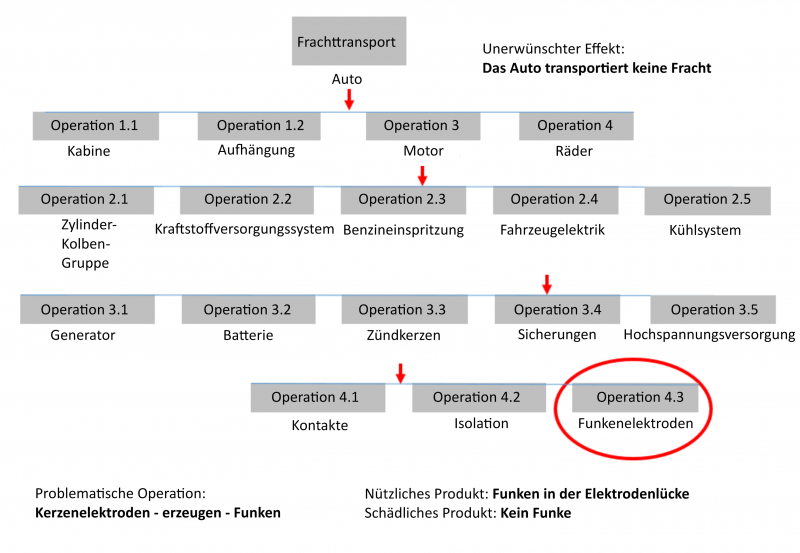
\includegraphics[width=.9\textwidth]{1212_xxl.png}\\[4pt]
  \textbf{Bild 3:} Hierarchisches Komponentenmodell.\\ Lokalisieren einer
  problembehafteten Komponente
\end{figure}

\subsection{Erste Phase: Analyse der Problemsituation}

Bei der Suche nach der Ursache eines Problems arbeitet sich ein erfahrener
Ingenieur (und auch jedes digitale Diagnoseprogramm) von der allgemeinen
Systemebene durch Analyse einzelner Komponenten und Unterkomponenten Schritt
für Schritt bis zum Ort des Problems vor (siehe Bild 3).  Diese Modellierung
ist als \emph{Analyse der Problemsituation} in der ersten Phase der
Problembearbeitung am TRIZ-Trainer auszuführen.  Dabei ist sowohl das TS zu
analysieren als auch dessen problembehaftete Komponente.  Dies bedeutet, dass
in der Regel \emph{zwei} Systemanalysen durchzuführen sind.

Zunächst ist das technische System (TS) abzugrenzen und dessen Zweck zu
bestimmen. Dazu wird das TS als Black Box durch einen \emph{Bezeichner}
(„sprechender Name“) grob abgegrenzt und dessen Zweck als \emph{primär
  nützliche Funktion} (PNF) benannt.  Die PNF ergibt sich aus dem Grund, warum
das untersuchte TS überhaupt existiert.  Dieser Grund erschließt sich, wenn
Ober- oder Nachbarsysteme identifiziert werden, für die der Dienst dieses TS
bedeutsam oder erforderlich ist.  In vielen Fällen ist er auch ohne eine
solche erweiterte Analyse ersichtlich.  Als dritter Bestandteil sind die
\emph{Betriebsbedingungen} des TS als Kontext grob zu fixieren.  Damit ist die
\emph{Spezifikation} des TS (grob) erfasst.

Um der Problematik der gestellten Aufgabe auf den Grund zu gehen, ist nun eine
genauere Analyse des TS als White Box erforderlich.  TRIZ geht vom Konzept
eines \emph{minimalen TS} und dessen grundlegendem Aufbau 
\begin{center}
  \normbox{Werkzeug} ---\normbox{bearbeitet}$\rightarrow$ \normbox{Objekt} 
\end{center}
aus.  Das \emph{Objekt} wird im Zuge dieser Bearbeitung in ein
\emph{nützliches Produkt} verwandelt.  Der (allgemeine) Zweck eines TS besteht
also darin, einen Arbeitsgegenstand in ein nützliches Ding zu verwandeln.

Diese Verwandlung erfordert allerdings einen energetischen und steuernden
Einfluss auf das Werkzeug oder allgemeiner das Arbeitsmittel.  Dieser Einfluss
erfolgt bei einfachen Werkzeugen direkt durch einen menschlichen Operator, in
komplexeren Kontexten aber indirekt durch weitere Komponenten. Im TRIZ-Trainer
wird dazu der Begriff der \emph{Maschine} in einem verallgemeinerten Sinn
(siehe Hilfesystem) verwendet, deren \emph{standardisierte Aufbauorganisation}
im Bild 4 gezeigt ist.
\begin{figure}[ht]\centering
  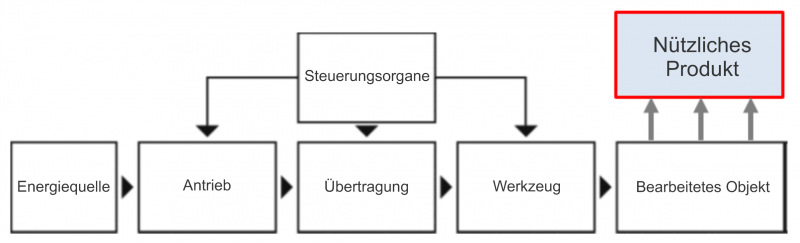
\includegraphics[width=.8\textwidth]{965_xxl.png}\\[4pt]
  \textbf{Bild 4:} Prinzipieller Aufbau einer „Maschine“
\end{figure}

Neben der \emph{Aufbauorganisation} (statisches Modell) ist für ein System
auch dessen \emph{Ablauforganisation} (dynamisches Modell) wichtig. Zur
Darstellung von Abläufen sind entsprechende Diagramme wie Sequenzdiagramme,
Zustandsdiagramme, Zustandsübergangsdiagramme, Prozessketten
usw.\ hilfreich. Die Abläufe im System verbinden Abläufe in den einzelnen
Komponenten, die auf Systemebene als \emph{elementar} betrachtet (und in
Diagrammdarstellungen in Unterdiagramme ausgelagert) werden, können neben dem
Aufruf von Funktionalität aber auch Zustandsänderungen an bearbeiteten
gemeinsamen \emph{Objekten} bewirken.  Komponenten sind in diesem Zusammenhang
Systemteile mit eigener aktiver Funktionalität, Ressourcen und Objekte passive
Targets funktionaler Transformationen. Der Objektbegriff unterscheidet sich
damit von dem der OO-Programmierung und folgt den Ansätzen eines „beyond
object oriented programming“, wie sie etwa in \cite{Szyperski2002} dargestellt
sind.

Ein einigermaßen vollständiges System umfasst nach \cite[S. 39]{TESE2018}
(siehe auch Bild 4) folgende Funktionalitäten:
\begin{itemize}[noitemsep]
\item die Funktionalität des operierenden Agenten (Arbeitsorgan, Werkzeug),
\item Energiebereitstellung (Energiequelle oder -speicher),
\item Antrieb (Umwandlung von Speicher- in Arbeitsenergie),
\item Transmission (Übretragung, Anpassung und Transport der Arbeitsenergie
  zum Arbeitsorgan) und
\item Steuerung.
\end{itemize}

\paragraph{Bearbeitungsrichtlinie für die erste Phase.}
Für die Modellierung der Gegebenheiten der Aufgabenstellung sind also in der
ersten Phase zu identifizieren 
\begin{enumerate}\itemsep0pt
\item das \emph{System} (als „sprechender Name“), dessen \emph{Zweck}, die
  \emph{PNF}, die erforderlichen \emph{Betriebsbedingungen} und die
  abzustellenden \emph{problematischen Wirkungen} (Abschnitt „Prä\-zi\-sierung
  der Umstände“),
\item die Aufbauorganisation des Systems nach dem im Bild 4 dargestellten
  Pattern -- welche Komponenten und welche Ressourcen werden genutzt, wo
  konzentriert sich das Problem, rekursive Analyse der Aufbauorganisation von
  Teilkomponenten wie in Bild 3 bis hin zur \emph{operativen Zone}, in der
  sich das Problem manifestiert -- (Abschnitt „Maschine“),
\item die Ablauforganisation des Systems als Ganzes (Vorarbeit zur
  Identifizierung von Ressourcen, die im System zur Lösung des Problems
  verfügbar sind) sowie der problematischen Teilkomponente (Abschnitt „Wie die
  Maschine arbeitet).
  
  Die Ablauforganisation führt in vielen Fällen auf eine klare Unterscheidung
  verschiedener \emph{Zustände}, die für optimale Lösungen in der Modellierung
  über verschiedene Betriebsmodi im System zu berücksichtigen sind.  Diese
  Zustände sind im Abschnitt „Wie die Maschine arbeitet“ klar begrifflich
  abzugrenzen.
\end{enumerate}

\paragraph{Zu 1. Typische Identifizierungen in einzelnen Aufgaben:}
\begin{itemize}[noitemsep]
\item Schiffsmast: Zweck Wasserstraßenverkehr, System Boot.
\item Güterzug anfahren: Zweck Gütertransport auf der Schiene, System
  Güterzug. 
\item Kipper im Bergbau: Zweck Erztransport aus der Grube, System
  Kipper. 
\end{itemize}

Am Ende dieser Analyse sind die nützlichen sowie die unzureichenden oder
schädlichen Wirkungen möglichst als formalisierte Aussagen
\begin{center}
  Werkzeug -- bearbeitet -- Objekt
\end{center}
aufzulisten („systemisch relevante Wirkungen“) und auf dieser Basis der
Konflikt (Ort, Zeit, Struktur) genauer zu beschreiben als Basis für die
Planung einer Transformation des Systems, welche das Problem löst. 

Am Ende dieser ersten Phase (in der Informatik auch als
\emph{Anforderungsanalyse} bezeichnet) steht ein genaues Modell des Systems.
Weiter ist (Abschnitt „Hypothesen aufstellen“) auf der Basis dieser genauen
Modellkenntnis eine \emph{präzisierte Aufgabe} zu formulieren, deren Umsetzung
das Problem lösen würde. Im Gegensatz zu Analysemethoden wie \emph{Design
  Thinking}, die stark auf die Wünsche des Kunden, aber weniger auf die
technischen Gegebenheiten ausgerichtet sind, wird durch die systematische
Modellierung ein gutes Verständnis für die technischen Gegebenheiten
erarbeitet und damit der zu analysierende Lösungsraum \emph{begründet} massiv
fokussiert im Gegensatz zum Brainstorming, das zu einer \emph{unbegründeten}
Fokussierung und zu einer „traditionellen“ Lösung ohne erfinderisches
Potenzial führt.  Diese stark fokussierende Wirkung einer TRIZ-Analyse auf
\emph{praktisch} Umsetzbares wird von Anwendern immer wieder als großer
Vorteil dieser Methodik hervorgehoben.  Mit der Formulierung der Aufgabe ist
die \emph{Richtung} der Lösung an dieser Stelle bereits klar, auch wenn die
Details im weiteren Prozess noch ausgearbeitet werden müssen.

\paragraph{Wie „radikal“ darf eine Lösung sein?}
In der Regel kann im Lösungsprozess das System so modifiziert werden, dass es
seine PNF weiter erfüllt wie bisher spezifiziert oder nur unwesentliche
Modifikationen vorgenommen werden müssen, sich die Transformation der
Ablaufstrukturen also \emph{lokal eingrenzen} und auf den Kontext des Systems
selbst beschränken lässt.  In anderen Aufgaben geht es um eine temporär
zusätzliche Funktion des Systems, die in einem anderen Systemzustand
auszuführen ist. Auch in diesem Fall ist die Analyse der PNF wichtig, da über
diese Funktion die verfügbaren Systemressourcen identifiziert werden, die auch
für die zusätzliche Funktion genutzt werden können (und sollten).

\paragraph{Wie „willkürlich“ ist die initiale Systembestimmung?}
Die anfängliche Systemeingrenzung stellt ein gewisses Willkürmoment eines
Trennens von „innen“ und „außen“ dar.  Es kann sein, dass sich während der
weiteren Modellierung herausstellt, dass ein anderer Detailgrad als System
angemessener ist.  Dann sollte die Modellierung auf jenem Level wiederholt
werden.  Mehr dazu finden Sie im Abschnitt „AIPS-2015“ des Hilfesystems.
Hilfreich ist es hierbei auch, die Ausführungen in (Koltze/Souchkov 2017,
Kapitel 4.3) zum Zusammenhang zwischen technischen (TW) und
physikalischen\footnote{Das ist verallgemeinernd zu verstehen, denn es gibt
  auch Widersprüche mit chemischem, biologischem usw. Hintergrund.}  (PW)
Widersprüchen zu beachten und zu einem (gelegentlich offensichtlichen) PW die
TW zu rekonstruieren, um zu verstehen, wie der PW im Gesamtsystem der
Modellierung einzubetten ist.

Vorausgesetzt werden natürlich auch elementare Kenntnisse zu naturgesetzlichen
Begriffen und Zusammenhängen, die Ihnen aus der Schule geläufig sein
sollten\footnote{Etwa Zusammenhänge zwischen verschiedenen Energieformen, zu
  Kräften, Momenten, Bewegungsgrößen usw.}.

\subsection{Zweite Phase: Lösung der Aufgabe}

Zur spezifizierten Hypothese werden in der \emph{zweiten Phase der Lösung}
durch genaue Analyse der verfügbaren Ressourcen eine oder mehrere
\emph{Lösungsideen} gefunden. Am Ende ist eine der Lösungsideen zur
\emph{finalen Lösung} genauer auszuarbeiten und zu prüfen, ob die Lösung auch
funktioniert.

Diese Phase umfasst folgende Teile:
\begin{itemize}[noitemsep]
\item [(1)] Auswahl eines \emph{Aufgabenmodells}, das auf die in der ersten
  Phase identifizierte Konfliktstruktur passt.
\item [(2)] Möglichst umfassende Identifizierung von \emph{Ressourcen}, die
  zum Aufgabenmodell und zur Konfliktstruktur passen.
\item [(3)] Auswahl eines geeigneten TRIZ-Werkzeugs als
  \emph{Umwandlungsmethode}. 
\item [(4)] Konfiguration des Werkzeugs entsprechend der konkreten
  Konfliktstruktur (\emph{Lösungs\-modell}).
\item [(5)] Instrumentierung des Lösungsmodells mit geeigneten Ressourcen.
\end{itemize}
Während (1) mit einer wesentlichen methodischen Entscheidung verbunden ist,
hängen die Schritte (2)-(5) eng zusammen. Ein stimmiges Bild des
instrumentierten Lösungsmodells ergibt sich oftmals erst nach mehrfachem Hin
und Her, wenn spätere neue Einsichten Einfluss auf frühere Schritte haben.
Meist wird dabei festgestellt, dass Modellierungen zu grob ausgeführt oder
wesentliche Aspekte übersehen wurden. Die Modellierung muss deshalb in einem
solchen Fall von jener Stelle an überarbeitet werden.

Es kann sich bei diesen Verfeinerungen auch herausstellen, dass die erste
Phase ungenügend ausgearbeitet wurde oder das Aufgabenmodell nicht passt.
Dann sollte mit den vertieften Einsichten in erste Phase zurückgekehrt, die
dortige Modellierung präzisiert und damit der Kontext adjustiert werden, der
für die zweite Phase konstitutiv ist.

Da dieser Teil im Hilfesystem sehr genau beschrieben ist, kann hier auf
weitere Erläuterungen verzichtet werden.

\subsection{Dritte Phase: Finale Lösung auswählen}

\paragraph{Eigene Lösungsansätze bewerten.}
TRIZ-Beratungsunternehmen überlassen die Auswahl der Lösung meist dem Kunden,
da in die Entscheidung oft auch weitere Anforderungen einfließen, die sich aus
betriebsinternen Abläufen ergeben.  Deshalb konzentriert sich die Beratung
nicht darauf, eine einzige starke Lösung zu finden, die unter bestimmten
Bedingungen wahrscheinlich schwierig zu implementieren ist, sondern bietet
eine Reihe von (begründeten) Lösungen, aus denen der Kunde die für ihn am
besten geeignete, lokal ideale Lösung kombinieren kann.
 
Dieser Ansatz wird auch im TRIZ-Trainer verfolgt, auch wenn wir hier keinen
\emph{Kunden} als Quelle der Probleme und zur Evaluierung der Lösungen haben.
Dementsprechend kann auch nur bedingt aus mehreren die beste Lösung ausgewählt
werden -- diejenige, die auf Grund allgemeiner Erfahrung und Logik als die
beste erscheint. Wenn Sie zu mehreren Lösungsvorschlägen gelangen, können Sie
im letzten Schritten der Vorlage (Schlussfolgerung, endgültige Entscheidung)
die Ihrer Meinung nach am besten funktionierende Lösung hervorheben und (mit
Begründung) als die effektivste herausstellen.  Als Bewertungskriterium sollte
die Frage untersucht werden, in welchem Umfang für die Lösung Änderungen am
vorhandenen System erforderlich sind -- optimal sind Lösungen, die nur geringe
Änderungen am Ort des Konflikts oder in dessen Nähe erfordern.

\paragraph{Wie genau muss die finale Lösung ausgearbeitet sein?}
Die finale Lösung muss so weit durchgearbeitet sein, dass auch sekundäre
Probleme gelöst sind.  Mit einer Lösung, die nur im Prinzip funktioniert, die
aber, wenn man versuchen würde, sie zu implementieren, auf weitere Hindernisse
stößt oder teuer oder kompliziert oder zu 99\% unrealistisch bzgl. der
Ressourcenanforderungen ist, kann man nicht zufrieden sein.  In diesem Fall
wird die Lösung zur Überarbeitung zurückgegeben mit folgenden zwei Optionen:
\begin{itemize}
\item Sie bleiben in Phase 2 und durchlaufen den Lösungszyklus erneut mit den
  erweiterten Kenntnissen und derselben Hypothese (Iteration).
  
  Modifizieren Sie das Aufgabenmodell oder verwenden Sie ein anderes, führen
  Sie noch einmal die Lösungsschritte aus und reichen die neue Lösung zur
  Bewertung ein.
\item Sie kehren in Phase 1 zurück, gehen anders an die Modellierung heran,
  formulieren eine neue Hypothese oder wählen eine andere aus den vorher
  schon aufgestellten mehreren Hypothesen aus und durchlaufen dann Phase 2
  noch einmal mit dem neuen  Ansatz.
\end{itemize}

\bibliographystyle{plain}
\begin{thebibliography}{xxx}
\bibitem{KS2017} Karl Koltze, Valeri Souchkov (2017). Systematische
  Innovation.  2. Auf"|lage, Hanser, München.  ISBN: 978-3-446-45127-8.

  Als E-Book im Uni-Netz verfügbar
  \url{http://dx.doi.org/10.3139/9783446452572}.
\bibitem{TESE2018} Alex Lyubomirskiy, Simon Litvin, Sergei Ikovenko et al.
  (2018).  Trends of Engineering System Evolution (TESE).  TRIZ Consulting
  Group. ISBN 978-3-00-059846-3.
\bibitem{Szyperski2002} Clemens Szyperski (2002). Component Software. Addison
  Wesley, Boston. 
\end{thebibliography}

\end{document}
